\section{分布函数}
\label{sec:rvd-distribution-functions}

分布要对许多集合给出概率。骰子只有六个取值，列一张表就够了；等待时间可以取任何非负实数，不可能把每个区间的概率逐一列出。能不能用一个实变量的函数记下全部信息？

\paragraph{累计到阈值的概率}
设想沿实轴从左向右移动一个阈值$x$，每到一处就问：取值不超过$x$的概率有多大？按质量的图景，这是阈值左侧（含阈值本身）累积的质量。阈值移动时，这个数只增不减，从$0$开始，最后到$1$。

\begin{definition}[分布函数]
\label{def:rvd-cdf}
随机变量$X$的\term{分布函数}（cumulative distribution function）定义为
\begin{equation}
  F_X(x)=\mathbb{P}(X\leq x),\qquad x\in\mathbb{R}.
  \label{eq:rvd-cdf}
\end{equation}
\end{definition}

分布函数对每个实数$x$都有定义，不论$X$实际取哪些值。只要知道它，左开右闭区间的概率就能算出。设$a<b$，事件$\{X\leq b\}$是互斥的$\{X\leq a\}$与$\{a<X\leq b\}$之并，由可加性
\[
  \mathbb{P}(X\leq b)=\mathbb{P}(X\leq a)+\mathbb{P}(a<X\leq b),
\]
移项得到
\begin{equation}
  \mathbb{P}(a<X\leq b)=F_X(b)-F_X(a).
  \label{eq:rvd-interval}
\end{equation}
区间取左开右闭，正好与定义中的“$\leq$”配套：$\{X\leq a\}$含$a$，减去之后右边的区间就不含$a$。

\paragraph{抽检中的次品数}
一批$5$件产品中有$2$件次品，不放回地随机抽取$2$件，记次品数为$X$。按第~\ref{chap:classical-probability}章的计数，无序抽法共$\binom52=10$种，等可能。两件都合格有$\binom32=3$种，一件次品一件合格有$2\times3=6$种，两件都是次品有$1$种。于是
\[
  \mathbb{P}(X=0)=0.3,\quad \mathbb{P}(X=1)=0.6,\quad \mathbb{P}(X=2)=0.1 .
\]

现在让阈值$x$扫过实轴。$x<0$时没有任何可能取值不超过$x$；$0\leq x<1$时只有取值$0$满足；$1\leq x<2$时取值$0$和$1$满足；$x\geq2$时全部满足。所以
\begin{equation}
  F_X(x)=\begin{cases}
    0,&x<0,\\
    0.3,&0\leq x<1,\\
    0.9,&1\leq x<2,\\
    1,&x\geq 2.
  \end{cases}
  \label{eq:rvd-inspection-cdf}
\end{equation}
图~\ref{fig:rvd-inspection-cdf}以$x=1.5$为例：(a)中红线左侧的柱子是被累计的质量，(b)中红点是它们的和$F_X(1.5)=0.9$。

\begin{BookInlineFigure}
  \centering
  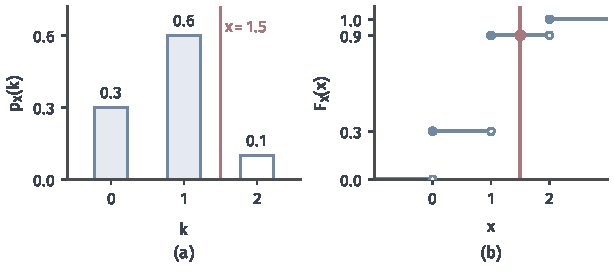
\includegraphics[width=104mm]{figures/07-probability/01-elementary-probability/matplotlib/rvd-inspection-cdf/figure.pdf}
  \caption{抽检次品数$X$的分布函数。(a)$X$取$0,1,2$的概率，红线是阈值$x=1.5$，左侧浅蓝柱被累计，右侧白柱不计；(b)分布函数，实心点是函数值，空心点是从左侧逼近的极限。红点$F_X(1.5)=0.3+0.6=0.9$。}
  \label{fig:rvd-inspection-cdf}
\end{BookInlineFigure}

$F_X$是阶梯函数：在两个可能取值之间，阈值移动不会越过新的质量，函数保持水平；阈值越过一个可能取值时，函数跳升，跳升的高度正是该处的概率。注意每个台阶的左端是实心点：$F_X(1)=0.9$，因为$\{X\leq1\}$包含$X=1$。

\paragraph{等待时间}
等待时间$T$（单位：分钟）不能列表，我们直接用分布函数给出模型：
\begin{equation}
  F_T(t)=\begin{cases}0,&t<0,\\1-\mathrm{e}^{-t},&t\geq0.\end{cases}
  \label{eq:rvd-waiting-cdf}
\end{equation}
它等价于规定“等待超过$t$分钟的概率是$\mathrm{e}^{-t}$”，等待越久越罕见。为什么这种形式适合描述等待，留到第~\ref{chap:common-distributions}章说明，这里只把它当作给定的模型。由式~\eqref{eq:rvd-interval}，等待$1$到$2$分钟的概率是
\[
  \mathbb{P}(1<T\leq2)=(1-\mathrm{e}^{-2})-(1-\mathrm{e}^{-1})=\mathrm{e}^{-1}-\mathrm{e}^{-2}\approx0.2325 .
\]
等待超过$2$分钟的概率是$1-F_T(2)=\mathrm{e}^{-2}\approx0.1353$。

这条曲线处处连续，没有跳跃。与抽检的阶梯对比，可以预料：跳跃对应集中在单点的概率，而等待时间没有哪一个具体时刻带有正概率。下面把这个预料写成定理。

\paragraph{分布函数的性质}
阶梯函数和连续曲线看起来很不同，但它们有共同的骨架：单调不减，在每一点从右侧连续，两端分别趋于$0$和$1$，跳跃高度等于单点概率。先对取有限或可数个值的随机变量证明这些性质；用密度给出的模型在第~\ref{sec:rvd-mass-density}节核验，一般情形的依据在第~\ref{chap:probability-spaces}章给出。

设$X$只取值$x_1,x_2,\dots$（有限个或可数个，互不相同），记$q_i=\mathbb{P}(X=x_i)$，这些数非负，总和为$1$。取有限个值时，每个事件的概率就是其中各取值概率之和；取可数个值时，我们把这一点作为模型的规定：$\mathbb{P}(X\in B)$等于$x_i\in B$的那些$q_i$之和。非负项级数可以任意重排和分组而和不变，所以这样规定的概率同样满足可加性。于是
\[
  F_X(x)=\sum_{i:\,x_i\leq x}q_i .
\]

\begin{theorem}[分布函数的性质]
\label{thm:rvd-cdf-properties}
设随机变量$X$只取有限或可数个值，$F=F_X$。则
\begin{enumerate}
  \item 单调不减：$x<y$时$F(x)\leq F(y)$；
  \item 右连续：对每个$x$，$\lim_{h\downarrow0}F(x+h)=F(x)$；
  \item 两端极限：$\lim_{x\to-\infty}F(x)=0$，$\lim_{x\to+\infty}F(x)=1$；
  \item 左极限存在，并且
  \begin{equation}
    F(x^{-})=\lim_{h\downarrow0}F(x-h)=\mathbb{P}(X<x),\qquad F(x)-F(x^{-})=\mathbb{P}(X=x).
    \label{eq:rvd-jump}
  \end{equation}
\end{enumerate}
\end{theorem}

\begin{proof}
单调性：$x<y$时，满足$x_i\leq x$的下标都满足$x_i\leq y$，后者的和多出一些非负项，所以$F(x)\leq F(y)$。

其余三条都依靠同一个估计：总和为$1$的级数，尾部可以任意小。给定$\varepsilon>0$，取$N$使
\[
  \sum_{i>N}q_i<\varepsilon .
\]
这时只有前$N$个取值可能带来不小的概率，而有限个点总是离给定的点有正的距离。

右连续：$F(x+h)-F(x)$是落在$(x,x+h]$里的那些$q_i$之和。前$N$个取值中大于$x$的有有限个，记它们到$x$的最小距离为$\delta>0$（若没有这样的取值，取$\delta=1$）。当$0<h<\delta$时，前$N$个取值都不在$(x,x+h]$中，于是
\[
  0\leq F(x+h)-F(x)\leq\sum_{i>N}q_i<\varepsilon .
\]

两端极限：当$x$小于$x_1,\dots,x_N$中的最小者时，$F(x)$只含下标大于$N$的项，所以$F(x)<\varepsilon$。当$x$不小于其中最大者时，$F(x)$包含前$N$项，所以
\[
  F(x)\geq\sum_{i\leq N}q_i>1-\varepsilon .
\]
又$0\leq F\leq1$，两端极限分别为$0$和$1$。

左极限：$F(x)-F(x-h)$是落在$(x-h,x]$里的$q_i$之和，它等于$\mathbb{P}(X=x)$加上落在$(x-h,x)$里的那些项。与右连续的论证相同，$h$足够小时后者小于$\varepsilon$，所以
\[
  \lim_{h\downarrow0}\bigl(F(x)-F(x-h)\bigr)=\mathbb{P}(X=x).
\]
移项即得式~\eqref{eq:rvd-jump}中左极限的值$F(x)-\mathbb{P}(X=x)=\mathbb{P}(X<x)$。
\end{proof}

右连续而不一定左连续，原因在于“$\leq$”包含阈值本身。图~\ref{fig:rvd-jump-limits}放大了抽检例子在$x=1$处的跳跃。从右侧逼近时，阈值$1+1/n$与$1$之间没有可能取值，累计的总是$X=0$和$X=1$两份质量，函数值恒为$0.9=F(1)$。从左侧逼近时，阈值$1-1/n$还没有越过$1$，累计的只有$X=0$那一份，极限是$0.3$。两者之差$0.6$就是$X=1$的概率。

\begin{BookInlineFigure}
  \centering
  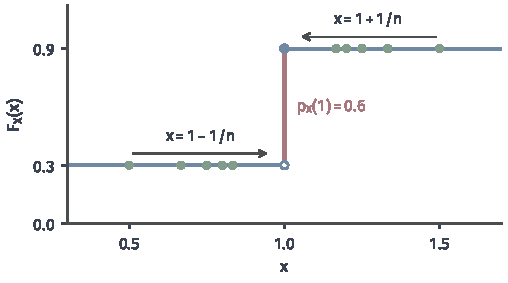
\includegraphics[width=86mm]{figures/07-probability/01-elementary-probability/matplotlib/rvd-jump-limits/figure.pdf}
  \caption{抽检次品数的分布函数在$x=1$处的两侧极限。绿点是阈值$1+1/n$与$1-1/n$（$n=2,\dots,6$）处的函数值：右侧一列恒为$0.9$，等于$F_X(1)$（实心点）；左侧一列恒为$0.3$，等于左极限（空心点）。红色竖线是跳跃高度$0.6=\mathbb{P}(X=1)$。}
  \label{fig:rvd-jump-limits}
\end{BookInlineFigure}

\paragraph{三条性质各管什么}
单调、右连续、两端极限这三条性质，每一条都排除了一类不可能是分布函数的函数。拿抽检例子对照，可以看清它们各自的作用。

单调不减保证区间概率非负：由式~\eqref{eq:rvd-interval}，$F(b)-F(a)$是概率，不能为负。右连续是“$\leq$”这一约定的结果。若改用$G(x)=\mathbb{P}(X<x)$记录累计概率，抽检例子给出
\[
  G(x)=\begin{cases}0,&x\leq0,\\0.3,&0<x\leq1,\\0.9,&1<x\leq2,\\1,&x>2,\end{cases}
\]
它在每个跳跃点取左侧的值，是左连续的。$G$包含的信息与$F_X$相同，只是约定不同；本书统一使用“$\leq$”，因此分布函数总是右连续的。

两端极限保证质量既不从左侧漏走，也不在右侧缺失。设某台设备收到请求后，以概率$1/2$会响应，响应前的等待按式~\eqref{eq:rvd-waiting-cdf}的规律分布；以概率$1/2$永不响应。由全概率公式，等待不超过$t$分钟的概率是
\[
  H(t)=\tfrac12\bigl(1-\mathrm{e}^{-t}\bigr),\qquad t\geq0,
\]
它单调、连续，$t\to\infty$时却只趋于$1/2$。缺少的一半质量在“无穷远处”，响应时间不是一个实数值的随机变量。要用实值随机变量描述这台设备，就得另外记录“是否响应”，或者给等待设一个上限。

\paragraph{累计事件往往更好算}
第~\ref{sec:rvd-random-variables}节求两枚骰子较大点数$M$的概率时，先数的是$\{M\leq m\}$，用的正是分布函数。对一般的实数$x$，$\{M\leq x\}$要求两个点数都不超过$x$，所以
\[
  F_M(x)=\frac{\lfloor x\rfloor^{2}}{36},\qquad 0\leq x<6,
\]
$x<0$时为$0$，$x\geq6$时为$1$，其中$\lfloor x\rfloor$是不超过$x$的最大整数。再由式~\eqref{eq:rvd-jump}读跳跃高度，就回到$\mathbb{P}(M=m)=(2m-1)/36$。最大值、最小值这类变量，“都不超过”或“都超过”的事件可以直接计数，单点事件反而要分情形，这时先求分布函数更方便。

\paragraph{各种区间的概率}
有了左极限，端点开闭不同的区间都能用分布函数表示。式~\eqref{eq:rvd-jump}给出$\mathbb{P}(X<x)=F(x^{-})$，与式~\eqref{eq:rvd-interval}同样相减，得到表~\ref{tab:rvd-intervals}。它们的规律是：区间包含左端点$a$时减去$F(a^{-})$，不含时减去$F(a)$；包含右端点$b$时用$F(b)$，不含时用$F(b^{-})$。

\begin{BookInlineTable}
  \centering
  \begin{tabular}{ll@{\qquad}ll}
    \toprule
    事件 & 概率 & 事件 & 概率\\
    \midrule
    $a<X\leq b$ & $F(b)-F(a)$ & $a\leq X\leq b$ & $F(b)-F(a^{-})$\\
    $a<X<b$ & $F(b^{-})-F(a)$ & $a\leq X<b$ & $F(b^{-})-F(a^{-})$\\
    $X>a$ & $1-F(a)$ & $X\geq a$ & $1-F(a^{-})$\\
    \bottomrule
  \end{tabular}
  \caption{用分布函数表示区间概率，其中$a<b$，$F=F_X$，$F(a^{-})$是左极限。$F$在$a$、$b$处连续时，左右两列相同。}
  \label{tab:rvd-intervals}
\end{BookInlineTable}

在抽检例子中端点会造成差别。由式~\eqref{eq:rvd-inspection-cdf}，$F(1^{-})=0.3$，所以
\[
  \mathbb{P}(1\leq X\leq2)=F(2)-F(1^{-})=1-0.3=0.7,
\]
而
\[
  \mathbb{P}(1<X\leq2)=F(2)-F(1)=1-0.9=0.1 .
\]
前者包含$X=1$的$0.6$，后者不包含。等待时间的分布函数处处连续，左极限等于函数值，端点开闭不影响结果：
\[
  \mathbb{P}(1\leq T\leq2)=\mathbb{P}(1<T\leq2)\approx0.2325 .
\]

\paragraph{分布函数确定分布}
上面的计算表明，区间及其有限并的概率都能由分布函数得到，因此两个随机变量的分布函数相同，它们在这些集合上的概率就相同。反过来还有一个更强的事实：任何单调不减、右连续、两端极限为$0$和$1$的函数，都是某个随机变量的分布函数。这一结论需要构造一般的概率模型，在第~\ref{chap:probability-spaces}章证明。它意味着定理~\ref{thm:rvd-cdf-properties}的前三条性质恰好刻画了所有分布函数，本部分可以放心地直接用一个满足这三条的函数来规定模型，就像式~\eqref{eq:rvd-waiting-cdf}所做的那样。
